\documentclass[runningheads]{llncs}
\usepackage[T1]{fontenc}
\usepackage[utf8]{inputenc}
\usepackage{graphicx,amsmath,amssymb,booktabs,tabularx,array}
\usepackage{microtype}
\usepackage{xurl}
\usepackage[hidelinks]{hyperref}
\usepackage{tikz}
\usetikzlibrary{arrows.meta,positioning}
\newcolumntype{Y}{>{\raggedright\arraybackslash}X}
\newcommand{\code}[1]{\texttt{#1}}
\setlength{\emergencystretch}{1.5em}
\title{Image-Driven Plant-State Monitoring of Indoor Strawberries: A Prototype Implementation}
\titlerunning{Image-Driven Plant-State Monitoring: Candidate Manuscript}
\author{Martin Arthur Andersen}
\authorrunning{M. A. Andersen}
\institute{Halden, Norway}
\begin{document}
\maketitle
\begin{center}\small\textit{Candidate manuscript --- 16 September 2026. Not submitted.}\end{center}
\begin{abstract}
An indoor cultivation monitor must translate observations into information that a grower can inspect. This paper describes a strawberry-monitoring prototype that combines camera-derived colour measurements, a ThingML Plant State Model, and a Python monitoring component. The design separates image processing from state interpretation: measurements are communicated as events, while explicit states and guards encode assumptions about development and possible deterioration. We reconstruct the design from the author's master's thesis and examine a pinned version of its software repository. The thesis reports accelerated replay tests and qualitative responses to changing watering conditions. These historical observations are distinguished from the present source inspection and from four bounded software checks. The inspection identifies overlapping colour ranges, an incompatible colour-space configuration, loss of temporal information, and interface inconsistencies that prevent treating the preserved files as a verified end-to-end configuration. The contribution is a concrete implementation account and an analysis of the conditions required to interpret its outputs. The available evidence supports discussing the monitoring design, but not quantified growth-stage accuracy, diagnosis of watering stress, or agronomic benefit.
\keywords{Plant monitoring \and Digital twin prototype \and ThingML \and Image processing \and Indoor cultivation}
\end{abstract}

\section{Introduction}
A photograph of a cultivation environment and a statement about a plant's state are different kinds of information. A camera records visible appearance. An image-processing routine produces measurements determined by its configuration. A state model interprets those measurements using assumptions about development and elapsed time. Keeping these steps distinguishable is important when an operator must decide whether to inspect a plant or adjust its environment.

This paper presents the image-driven monitoring part of an indoor strawberry prototype developed in a master's project~\cite{thesis}. The project combined cameras, environmental sensors, image processing, a Plant State Model, and a Python monitoring program. Rather than learning plant-state labels from an annotated image collection, the selected approach extracted colour-region measurements and supplied them to an explicit state model. Its intended output was a report about development or a possible deviation requiring attention.

The research question is: \emph{How can image-derived colour measurements support explicit, state-based monitoring of indoor strawberry cultivation?} We address the question through the concrete decomposition and implementation of the prototype, not through a claim that its colour segmentation is a new algorithm. The paper contributes an account of the observation-to-state pipeline, a traceable description of its model and interfaces, and a critical examination of the evidence available for interpreting its outputs.

This thesis-derived account adds source inspection and bounded software checks, not a new cultivation experiment. Dates of the historical watering changes are unavailable for alignment with the recovered images. We therefore make no causal claim about detecting underwatering or overwatering.

Environmental forecasting remains system context only. Regression comparisons, sensor maintenance, energy use, and noise measurements are outside this paper's contribution.

\section{Context and Related Work}
Digital twins for cultivation can combine observations, models, and operator-facing information. Jans-Singh et al.~\cite{janssingh2020} describe an urban-integrated hydroponic farm in which wireless measurements and manual records inform a site-specific model and decision support. David et al.~\cite{david2023} discuss challenges and lessons from an industrial cyber-biophysical system in controlled-environment agriculture. These studies establish relevant application contexts; neither is an experimental comparator for the prototype considered here.

ThingML provides a modelling language and configurable code-generation framework for heterogeneous targets~\cite{harrand2016}. The present prototype uses it to express the stateful interpretation of measurements. Its use does not make the biological assumptions in a statechart correct: code generation and state-transition execution address software behaviour, whereas correspondence with plant development requires separate evidence.

Colour thresholding is an established image-processing operation. OpenCV documents conversion to HSV and range-based extraction of coloured regions~\cite{opencvcolour}. The choice here is to connect such measurements to explicit states and warnings. We do not report a comparison with neural-network classifiers or established phenotyping pipelines, and consequently make no claim of superior accuracy, computational efficiency, or annotation efficiency.

The strawberry cultivation system also appears in the later DarTwin/SysMLv2 work by Haugen et al.~\cite{dartwin2025}, where it serves as a modelling example in an investigation of language-extension and tooling capabilities. The shared case is acknowledged. The present account concerns the earlier monitoring implementation, its observation interfaces, and the limits of its preserved evidence; it does not claim the cultivation case or a new digital-twin modelling language as a novel contribution.

\section{System Design}
\subsection{Physical Setting and Intended Use}
The thesis describes a compact indoor grow tent, cameras observing plants from above and from the side, environmental sensing, lighting, ventilation, and irrigation equipment~\cite[Secs.~3.1 and 7.2]{thesis}. The image-processing part was intended to track changes in visible plant features. Environmental measurements supported a separate monitoring and forecasting path. Figure~\ref{fig:setting} shows an example frame already included in the public software repository; it is an illustration of the installation, not a reference annotation.

\begin{figure}[t]
\centering
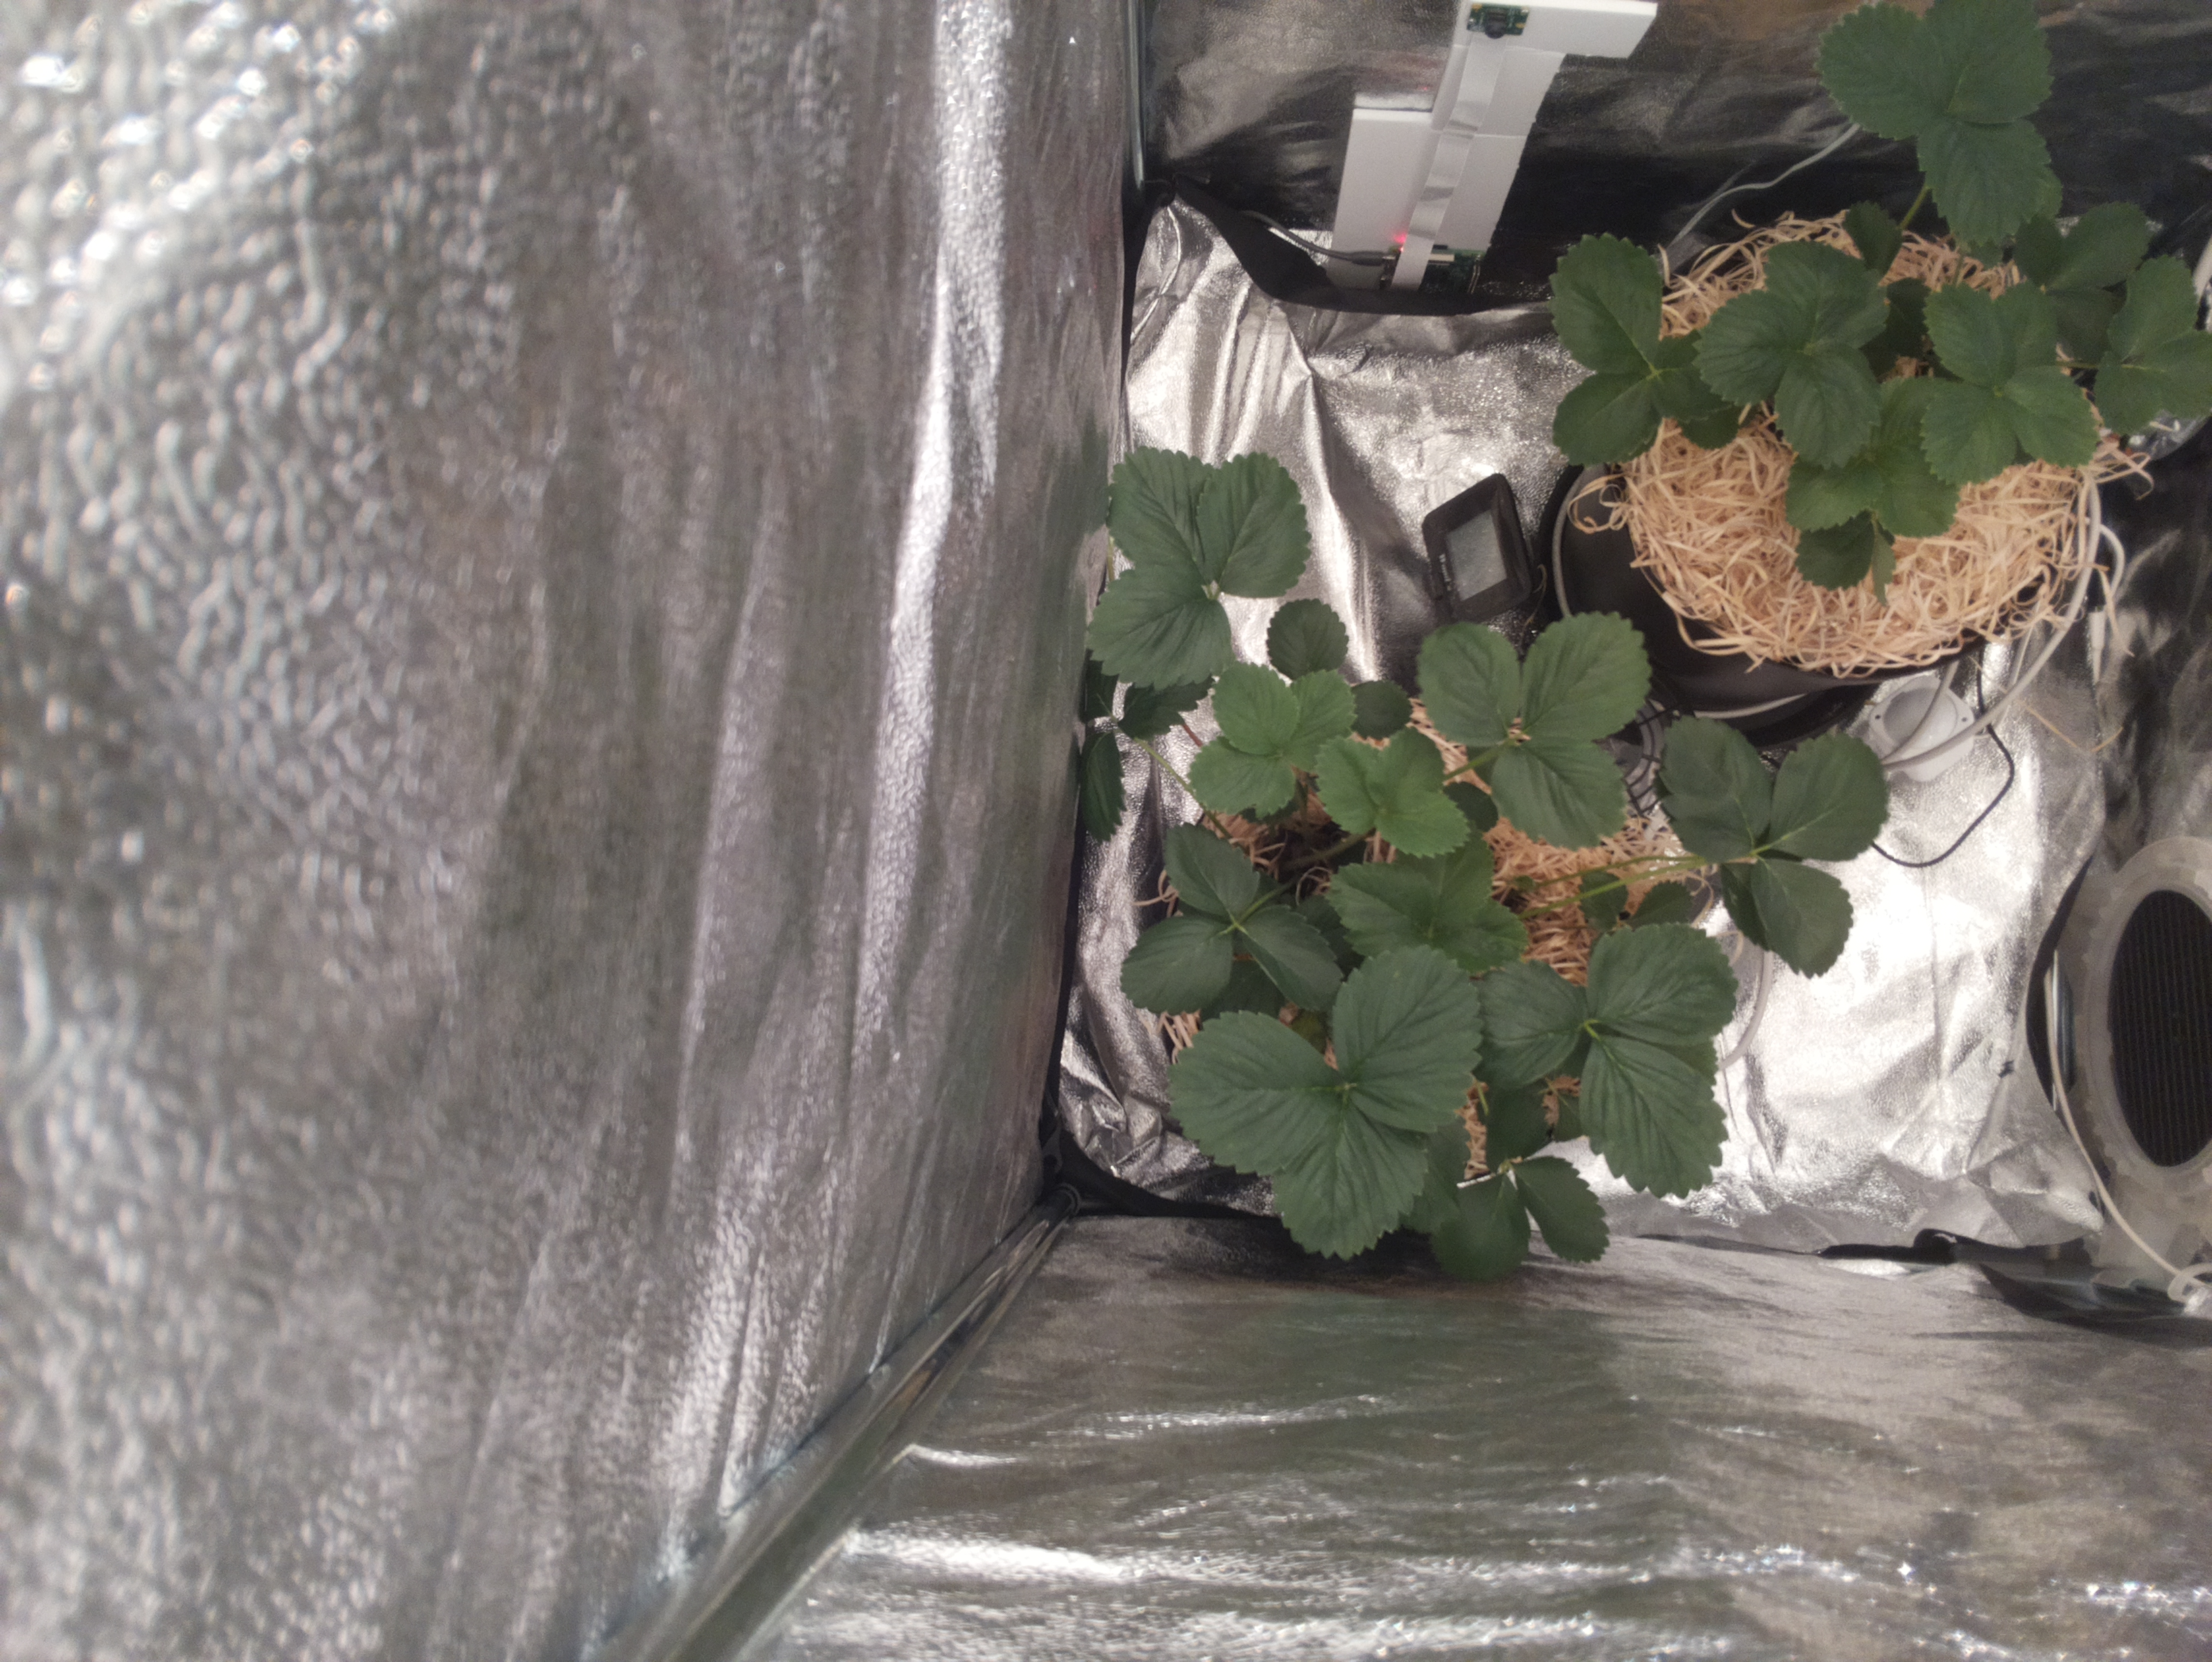
\includegraphics[width=.68\linewidth]{figures/cultivation.jpg}
\caption{Example cultivation image already distributed as \code{input.png} in the pinned repository~\cite{autotent}. The two visible pots illustrate the camera scene, not the number of independent plants or runs in the complete study. The image is not labelled as healthy, distressed, or a particular developmental stage.}
\label{fig:setting}
\end{figure}

The thesis's functional diagram places a human actuator at the receiving end of plant-state and environmental reports~\cite[Fig.~4.1]{thesis}. Although the installation included scheduled and remotely controllable equipment, the image-to-state path examined here does not establish automatic irrigation or lighting adjustment from a state transition. We describe the intended use as monitoring and support for human inspection. We retain the term \emph{digital twin prototype} as the thesis's designation, without claiming a validated physiological simulator or a demonstrated autonomous control loop.

\subsection{Software Decomposition}
Figure~\ref{fig:pipeline} summarizes the thesis's design. The image processor isolates configured colour regions and derives numerical features. The Plant State Model maintains a developmental interpretation and can report a distress-related state. The Python monitoring component associates states with environmental conditions and reports deviations. Acquisition, interpretation, and reporting have different responsibilities even when implemented on the same computer.

\begin{figure}[t]
\centering
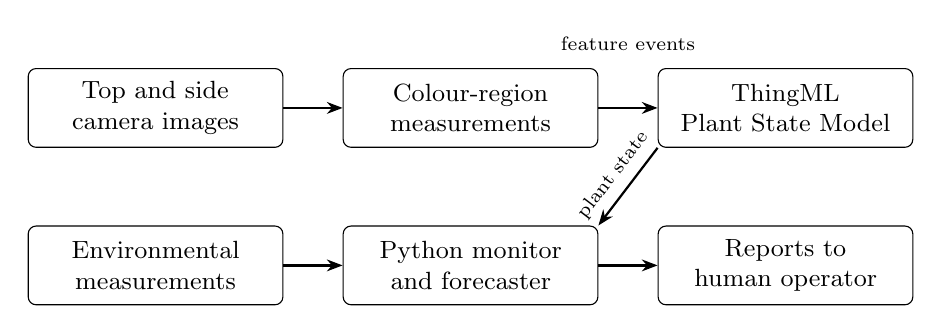
\begin{tikzpicture}[font=\small,box/.style={draw,rounded corners=1mm,align=center,minimum height=10mm,text width=30mm},arr/.style={-{Stealth[length=2mm]},thick}]
\node[box] (cam) at (0,0) {Top and side\\camera images};
\node[box] (feat) at (4,0) {Colour-region\\measurements};
\node[box] (state) at (8,0) {ThingML\\Plant State Model};
\node[box] (sensors) at (0,-2) {Environmental\\measurements};
\node[box] (mon) at (4,-2) {Python monitor\\and forecaster};
\node[box] (human) at (8,-2) {Reports to\\human operator};
\draw[arr] (cam)--(feat);
\draw[arr] (feat)--node[above=6mm,font=\scriptsize]{feature events}(state);
\draw[arr] (sensors)--(mon);
\draw[arr] (state.south west)--node[above,sloped,font=\scriptsize]{plant state}(mon.north east);
\draw[arr] (mon)--(human);
\end{tikzpicture}
\caption{Functional decomposition summarized from the thesis~\cite[Secs.~4.1--4.2 and Fig.~4.1]{thesis}. Arrows express the intended information flow, not a claim that the archived files have been executed together in this configuration. Environmental forecasting is context only and is not evaluated in this paper.}
\label{fig:pipeline}
\end{figure}

The decomposition separates acquisition, feature extraction, and state interpretation. The sender and receiver must nevertheless agree on feature names, units, region identifiers, topics, and timing; colocating their files in a repository does not establish these agreements.

\section{From Images to State Reports}
\subsection{Colour-Region Measurements}
The thesis describes cropping, colour-range selection, morphological operations, contour filtering, and export of measurements to CSV~\cite[Sec.~3.2.2]{thesis}. It calls the ranges RGB in that section and describes HSV conversion in Section~5.5.5. The inspected \code{grid\_count.py} converts the cropped image to HSV~\cite{autotent}. Table~\ref{tab:ranges} records its literal configuration rather than silently translating the thesis's terminology.

\begin{table}[t]
\caption{Green-channel bounds in the inspected \code{grid\_count.py}. Labels are preserved source names, not independently validated leaf-colour classes. Bounds are inclusive.}
\label{tab:ranges}
\centering
\begin{tabular}{lrrr}
\toprule
Source label & Hue & Saturation & Value\\
\midrule
\code{light\_green} & 30--90 & 85--255 & 30--255\\
\code{medium\_green} & 40--70 & 30--85 & 30--255\\
\code{dark\_green} & 30--90 & 30--85 & 30--255\\
\bottomrule
\end{tabular}
\end{table}

The script removes the rightmost 100 image columns, forms one mask per configured range, and applies closing followed by opening with a $7\times7$ kernel and two iterations for each operation. It then extracts external contours and retains those whose area exceeds an interactively supplied threshold $\tau$. The value returned under the name \code{total\_pixel\_count} is
\begin{equation}
 A_c(I)=\sum_{q\in C_c(I):\,\operatorname{area}(q)>\tau}\operatorname{area}(q),
 \label{eq:area}
\end{equation}
where $C_c(I)$ denotes the external contours after preprocessing for channel $c$. Equation~\ref{eq:area} describes the inspected implementation; it is not a new estimator. Summed contour area is not the same operation as counting non-zero mask elements. Similarly, the number of surviving contours is not necessarily a count of anatomically distinct leaves.

The medium-green bounds are contained within the dark-green bounds, so summing channels does not yield a unique total green area. Their names are not a calibrated ordering of leaf maturity. Camera distance, cropping, occlusion, background, and the area threshold affect the output. The thesis reports adjusting the threshold when camera distance changed~\cite[Sec.~3.2.2]{thesis}; the preserved material does not supply a complete, date-indexed configuration history.

The intended extension to red, yellow, and white was to provide evidence about flowers and berries. However, the separate \code{grid\_count\_rwy.py} uses HSV conversion together with lower hue bounds of 220 for white and 255 for red and yellow. Those bounds lie outside the documented standard 8-bit HSV hue range of 0--179~\cite{opencvcolour}. This configuration cannot support a verified flower/fruit detection claim as preserved. Correcting it would constitute a separately recorded implementation change, not reproduction of the archived configuration.

\subsection{The Plant State Model}
The model receives feature-related messages and updates an explicit state. The thesis's conceptual progression is germination, seedling, growth, and fruiting, with warnings when expected progress is absent or measurements suggest deterioration~\cite[Sec.~4.3]{thesis}. Table~\ref{tab:states} summarizes the intended interpretation. These are modelling assumptions, not biological ground-truth categories established by the present work.

\begin{table}[t]
\caption{Intended state interpretation in the thesis. This summarizes the design, not a verified transcription of every implementation guard.}
\label{tab:states}
\small
\begin{tabularx}{\linewidth}{@{}lYY@{}}
\toprule
State & Intended evidence & Interpretation boundary\\
\midrule
Germination & Initial state; timeout if expected progress does not occur. & Starting the program does not establish the actual age of a plant.\\
Seedling & Visible side-camera growth or configured green measurements. & Visibility and camera geometry affect the observation.\\
Growth & Green-region measurements associated with developing foliage. & Projected image area is not biomass or physiological health.\\
Fruiting & Additional colour evidence intended to indicate flowers or berries. & Colour alone does not establish the object or ripeness.\\
Distress-related & Timeout or a feature decline interpreted by a guard. & A warning does not identify the cause of a change.\\
\bottomrule
\end{tabularx}
\end{table}

The pinned ThingML source contains the states \code{Germination}, \code{Seedling}, \code{Growing}, and \code{Fruting}, with two distress-related states. The spelling \code{Fruting} is present in the source, while an emitted report uses \code{Fruiting}. The thesis's results section uses \emph{flowering} when listing the fourth stage. We preserve this distinction: a reported flowering transition is not silently reclassified as independently confirmed fruiting.

The implementation starts germination and seedling timers with durations of 10 and 14 days, respectively, and uses a configurable fruit-related threshold whose archived default is 10. It also creates two section sessions. These settings establish software configuration, not the number of independent biological experiments or validated agricultural timing limits~\cite{autotent}.

Some guards mix conjunction and disjunction without explicit grouping. In the growth-to-distress transition, an incoming \code{green\_pixel\_count} is compared with a stored \code{current\_light\_green\_pixel\_count}; the late-distress return transition also uses a less-than comparison. We do not replace these expressions with the intended rules in Table~\ref{tab:states} or claim their compiled behaviour has been established. Resolving the guard semantics and the relationship between model source and generated executable is a remaining implementation task.

\subsection{Messages, Reporting, and Replay}
The internal ThingML declaration represents an observation as
\begin{equation}
 \code{messages}(\mathrm{section\_id},\mathrm{msg\_type},\mathrm{msg\_txt},\mathrm{value}),
\end{equation}
and defines a separate $\code{reply}(\mathrm{id},\mathrm{content})$ message. The declaration contains no explicit capture timestamp~\cite{autotent}. This is relevant to replay: a model can receive the same numerical sequence at a different rate and experience different timer behaviour.

The thesis reports replaying CSV-derived MQTT messages five seconds apart and accelerating the germination and seedling timers by a factor of 1440~\cite[Sec.~5.5.2]{thesis}. We report those settings as documented; the available records do not establish that their combined time mapping preserved all original capture intervals. Missing dates cannot be treated as observed zero growth, and a daily filename is not evidence of uniformly spaced measurements.

The preserved files also expose interface differences. The image exporter writes human-readable CSV headers such as \code{Light\_green Total Pixel Count}. The inspected sender expects \code{light\_green\_pixel\_count} and defaults absent keys to zero. Its MQTT topic names differ from those in the ThingML platform-specific model, and the PIM's reply declaration differs from the PSM's receiving message declaration. The preserved files therefore require an identified adapter or reconciled configuration before end-to-end reproduction.

\section{Evidence and Observations}
\subsection{Evidence Sources and Method}
We distinguish three forms of evidence. First, the master's thesis records the historical design, tests, and observations. Second, the public repository is inspected at commit \code{814bb768aa99}; the complete identifier and file hashes are recorded in the accompanying evidence register~\cite{autotent}. Third, four small checks exercise values and operations transcribed from the inspected files. These checks are software-level examples, not experiments on plant-state accuracy.

Recovered camera material provides supplementary evidence that dated originals survive. The two inspected endpoint files are dated 5 July 2023 and 6 March 2024. This establishes neither uninterrupted coverage nor a count of valid observations. The July frame is byte-identical to the already-public example image used in Figure~\ref{fig:setting}. The later frame and private archive are not redistributed with this candidate.

The recovered capture script records a startup acquisition and subsequent daily acquisition at 07:59 in that version. It also writes a general acquisition message after attempting both cameras, even when one camera operation reports failure. The surviving log contains such partial-success cases. These observations justify distinguishing capture attempts from readable image files; they do not establish a complete failure rate for the archive. The script and log were inspected, not executed to contact the installation.

\subsection{Historical Results Reported in the Thesis}
The thesis reports 258 days of hourly environmental sensor data and six days of unusable image data associated with the lighting schedule~\cite[Sec.~6.1]{thesis}. It describes a change from a one-minute to a five-minute image-capture lighting interval. Its plant-state results refer to 252 days' worth of images~\cite[Sec.~6.4]{thesis}. We retain these as historical reported quantities, not a verified inventory of the recovered collection, and do not infer hourly image capture from hourly environmental sensing.

For the Plant State Model, the thesis reports expected transitions during replay, timeout-related distress indications, and the use of two initial messages when a scenario began with plants already in the growth stage. It also reports distress on the first day of a simulated underwatering scenario and a return to growth under improved conditions~\cite[Sec.~6.4]{thesis}. These are qualitative observations recorded by the developer. The source does not supply an independently annotated test set, per-class sample counts, or error estimates that would justify turning them into an accuracy percentage.

Figure~5.1 of the thesis associates green-measurement trajectories with optimal conditions, stopped watering, light watering, and overwatering~\cite[Sec.~5.1.1 and Fig.~5.1]{thesis}. The calendar dates of those interventions are not available for the recovered archive. Consequently, this figure documents the original experiment's interpretation, but it is not used here to label particular recovered photographs or to measure detection delay. Inferring treatment dates from the same colour decline used by the monitor would not provide an independent reference.

\subsection{Bounded Software Checks}
The supplementary checker exercises explicitly transcribed source fixtures without acquisition, actuation, broker communication, or model compilation. Table~\ref{tab:checks} reports the executed checks.

\begin{table}[t]
\caption{New software-level checks, not biological validation. Inputs are constructed fixtures derived from the inspected source configuration and operations.}
\label{tab:checks}
\small
\begin{tabularx}{\linewidth}{@{}lYY@{}}
\toprule
Check & Constructed input & Observed consequence\\
\midrule
Colour overlap & HSV value $(50,60,100)$ with the green bounds in Table~\ref{tab:ranges}. & Matches both medium-green and dark-green ranges.\\
Hue domain & Red, yellow, white, green, blue, and black RGB pixels converted to standard 8-bit HSV. & All six yield zero matches in every archived red/yellow/white range.\\
CSV hand-off & A non-zero row under the exporter-style headers, read with the sender's expected keys and defaults. & All three requested green measurements become zero.\\
Temporal plotting & Two channels $[7,0,9]$ and $[7,8,0]$ with the source's per-channel zero filtering. & Both become two-element series; their second elements represent different original observations.\\
\bottomrule
\end{tabularx}
\end{table}

The hue result is not evidence that the sampled plants had no flowers or fruit. It is the consequence of an incompatible configuration; the documented domain also rules out those hue lower bounds beyond the six example colours. The CSV result demonstrates a possible silent conversion of missing fields into apparent measurements. The plotting example shows why ordinal plot positions cannot establish calendar alignment after channel-specific filtering. The source also iterates over directory entries without explicit sorting, further limiting chronological interpretation of its unmodified plots.

These checks do not prove that the inspected configuration produced the historical results. Conversely, reported historical success does not establish consistency of the preserved files. End-to-end reproduction requires identification of the executed version and configuration.

\section{Discussion and Limitations}
\subsection{What the Prototype Contributes}
The design provides a concrete answer to the research question: colour measurements can be represented as named observations, supplied to a stateful model, and translated into reports alongside environmental monitoring. An explicit state model makes initialization, timeouts, transitions, and recovery rules inspectable. This is useful as an implementation structure, but its usefulness for growers has not been evaluated in a user study.

The case also shows why the distinction between measurements and interpretations matters. A decline in a colour-region measure may trigger a model rule, but the trigger does not reveal whether the cause was a change in plant appearance, camera position, illumination, segmentation configuration, or missing input. Distress-related state names should therefore be read as the model's classifications, not independently established diagnoses.

Three engineering implications follow from the inspected artefacts. A measurement record should retain its image identity, capture time, camera position, region, and configuration. Missing fields should remain distinguishable from numerical zero. Replay should have an explicit time mapping and an initialization procedure suitable for the observed sequence. These are recommendations from the present inspection, not features claimed to have been implemented in the historical prototype.

\subsection{Limits of the Evidence}
\textbf{Measurement validity.} There are no independent region masks or developmental reference labels in this candidate evaluation. Contour counts may merge overlapping leaves or include non-plant regions. Projected colour area is not calibrated physical leaf area. The overlapping ranges and incompatible flower/fruit configuration require attention before stronger interpretation is warranted.

\textbf{Historical reproducibility.} The thesis, inspected source snapshot, generated executable, recovered images, and capture configuration have not been linked into one verified execution history. RGB/HSV descriptions, the fourth state's terminology, message interfaces, and replay settings differ across sources. The checks preserve these discrepancies rather than silently repairing them. No current end-to-end ThingML/MQTT execution is claimed.

\textbf{Causality and generalization.} Missing intervention dates prevent treatment-aligned analysis. The recovered frame count and plant continuity have not been established, and repeated photographs are not independent growing experiments. The work cannot support generalization across strawberry varieties, cultivation sites, or disease conditions. It also cannot demonstrate improved yield, reduced water use, or better decisions.

\textbf{Study design.} The original method was developed during the same project that generated the images. A later split of that archive would not make it an independently collected validation dataset. The present checks examine a few definite software properties; they are neither a systematic test suite for the entire application nor an empirical estimate of monitoring effectiveness.

\section{Conclusion}
The indoor strawberry prototype illustrates a concrete approach to image-driven monitoring: extract configured colour-region measurements, communicate them as events, and interpret them through an explicit Plant State Model connected to operator-facing monitoring. The thesis provides qualitative historical observations; the preserved software makes assumptions and integration requirements inspectable. The present inspection and bounded checks expose conditions that must be resolved before claiming a reproducible end-to-end implementation. The contribution is therefore a prototype implementation account with explicit evidence limits, not a validated plant-health classifier or proof of agronomic benefit.

\subsubsection*{Availability and manuscript status.}
The historical software is public~\cite{autotent}; this candidate adds manuscript source, an evidence register, and bounded checks on a separate branch. Private images and logs are not released. Author review of metadata, authorship, venue, and implementation issues remains pending. Generative AI assisted drafting, source inspection, and preparation of the checks; this candidate has not been approved for submission.

\bibliographystyle{splncs04}
\bibliography{references}
\end{document}
